% !TEX root = ../main.tex
%-------------------------------------------------------------------------------
%-------------------------------------------------------------------------------
\begin{frame}\begin{center}
		\LARGE\textbf{Quantitative}
\end{center}\end{frame}
%-------------------------------------------------------------------------------
%-------------------------------------------------------------------------------
\begin{frame}\textbf{Alternatives}\vspace{0.3cm}

\begin{itemize}\setlength\itemsep{1em}
  \item variance-based
  \item moment-independent
  \item information-based
\end{itemize}

\end{frame}
%-------------------------------------------------------------------------------
%-------------------------------------------------------------------------------
\begin{frame}\begin{center}
		\LARGE\textit{Variance-based methods}
\end{center}\end{frame}
%-------------------------------------------------------------------------------
%-------------------------------------------------------------------------------
\begin{frame}
	\begin{align}\label{Variance decomposition}
	V[Y] = V_{X_i}[E_{X_{\sim i}}[Y\mid X_i]] + E_{X_i}[V_{\vec{X}_{\sim i}}[Y\mid X_i]]
	\end{align}
\end{frame}
%-------------------------------------------------------------------------------
%-------------------------------------------------------------------------------
\begin{frame}\textbf{Main effect}\vspace{0.3cm}

\begin{itemize}\setlength\itemsep{1em}
\item We rank all based on the smallest conditional variance $V[Y \mid X_i = x_i]$ evaluated over all possible vales $x_i$ of $X_i$. Following Equation (\ref{Variance decomposition}), this is equivalent to ranking factors by the largest
$V_{X_i}[E_{\vec{X}_{\sim i}}[Y\mid X_i]]$ and so the main effect is defined as:
\end{itemize}

\begin{align*}
S^M_i & = \frac{V_{X_i}[E_{\vec{X}_{\sim i}}[Y\mid X_i]]}{V[Y]}
\end{align*}
\end{frame}

%-------------------------------------------------------------------------------
%-------------------------------------------------------------------------------
\begin{frame}\textbf{Total effect}\vspace{0.3cm}

\begin{itemize}
\item We want to identify the factors that we can fix at their value without significantly reducing the output variance.
\end{itemize}

\begin{align*}
S^T_i & = \frac{E_{\vec{X} \sim i}[V_{X_i}[Y \mid \vec{X}_{\sim i}]]}{V[Y]} = 1 - S^M_{\sim i}
\end{align*}

\end{frame}
%-------------------------------------------------------------------------------
%-------------------------------------------------------------------------------
\begin{frame}\begin{center}
		\LARGE\textit{Ishigami function}

		\begin{align*}
				f(\vec{x}) = \sin(x_1) + a\, \sin^2 (x_2) + b\, x_3^4\, \sin(x_1)
		\end{align*}

\end{center}\end{frame}
%-------------------------------------------------------------------------------
%-------------------------------------------------------------------------------
\begin{frame}

	\begin{itemize}\setlength\itemsep{1em}
		\item The Ishigami function of \citeA{Ishigami.1990} is used as an example for uncertainty and sensitivity analysis methods, because it exhibits strong nonlinearity and nonmonotonicity.

		\item It also has a peculiar dependence on $x_3$, as described by \citeA{Sobol.1999}.

		 \item The independent distributions of the input random variables are usually: $x_i \sim Uniform[-\pi, \pi]$, for all $i = 1, 2, 3$.
	\end{itemize}

\end{frame}
%-------------------------------------------------------------------------------
%-------------------------------------------------------------------------------
\begin{frame}
\begin{figure}[htp]\centering\caption{Uncertainty propagation}
\scalebox{0.30}{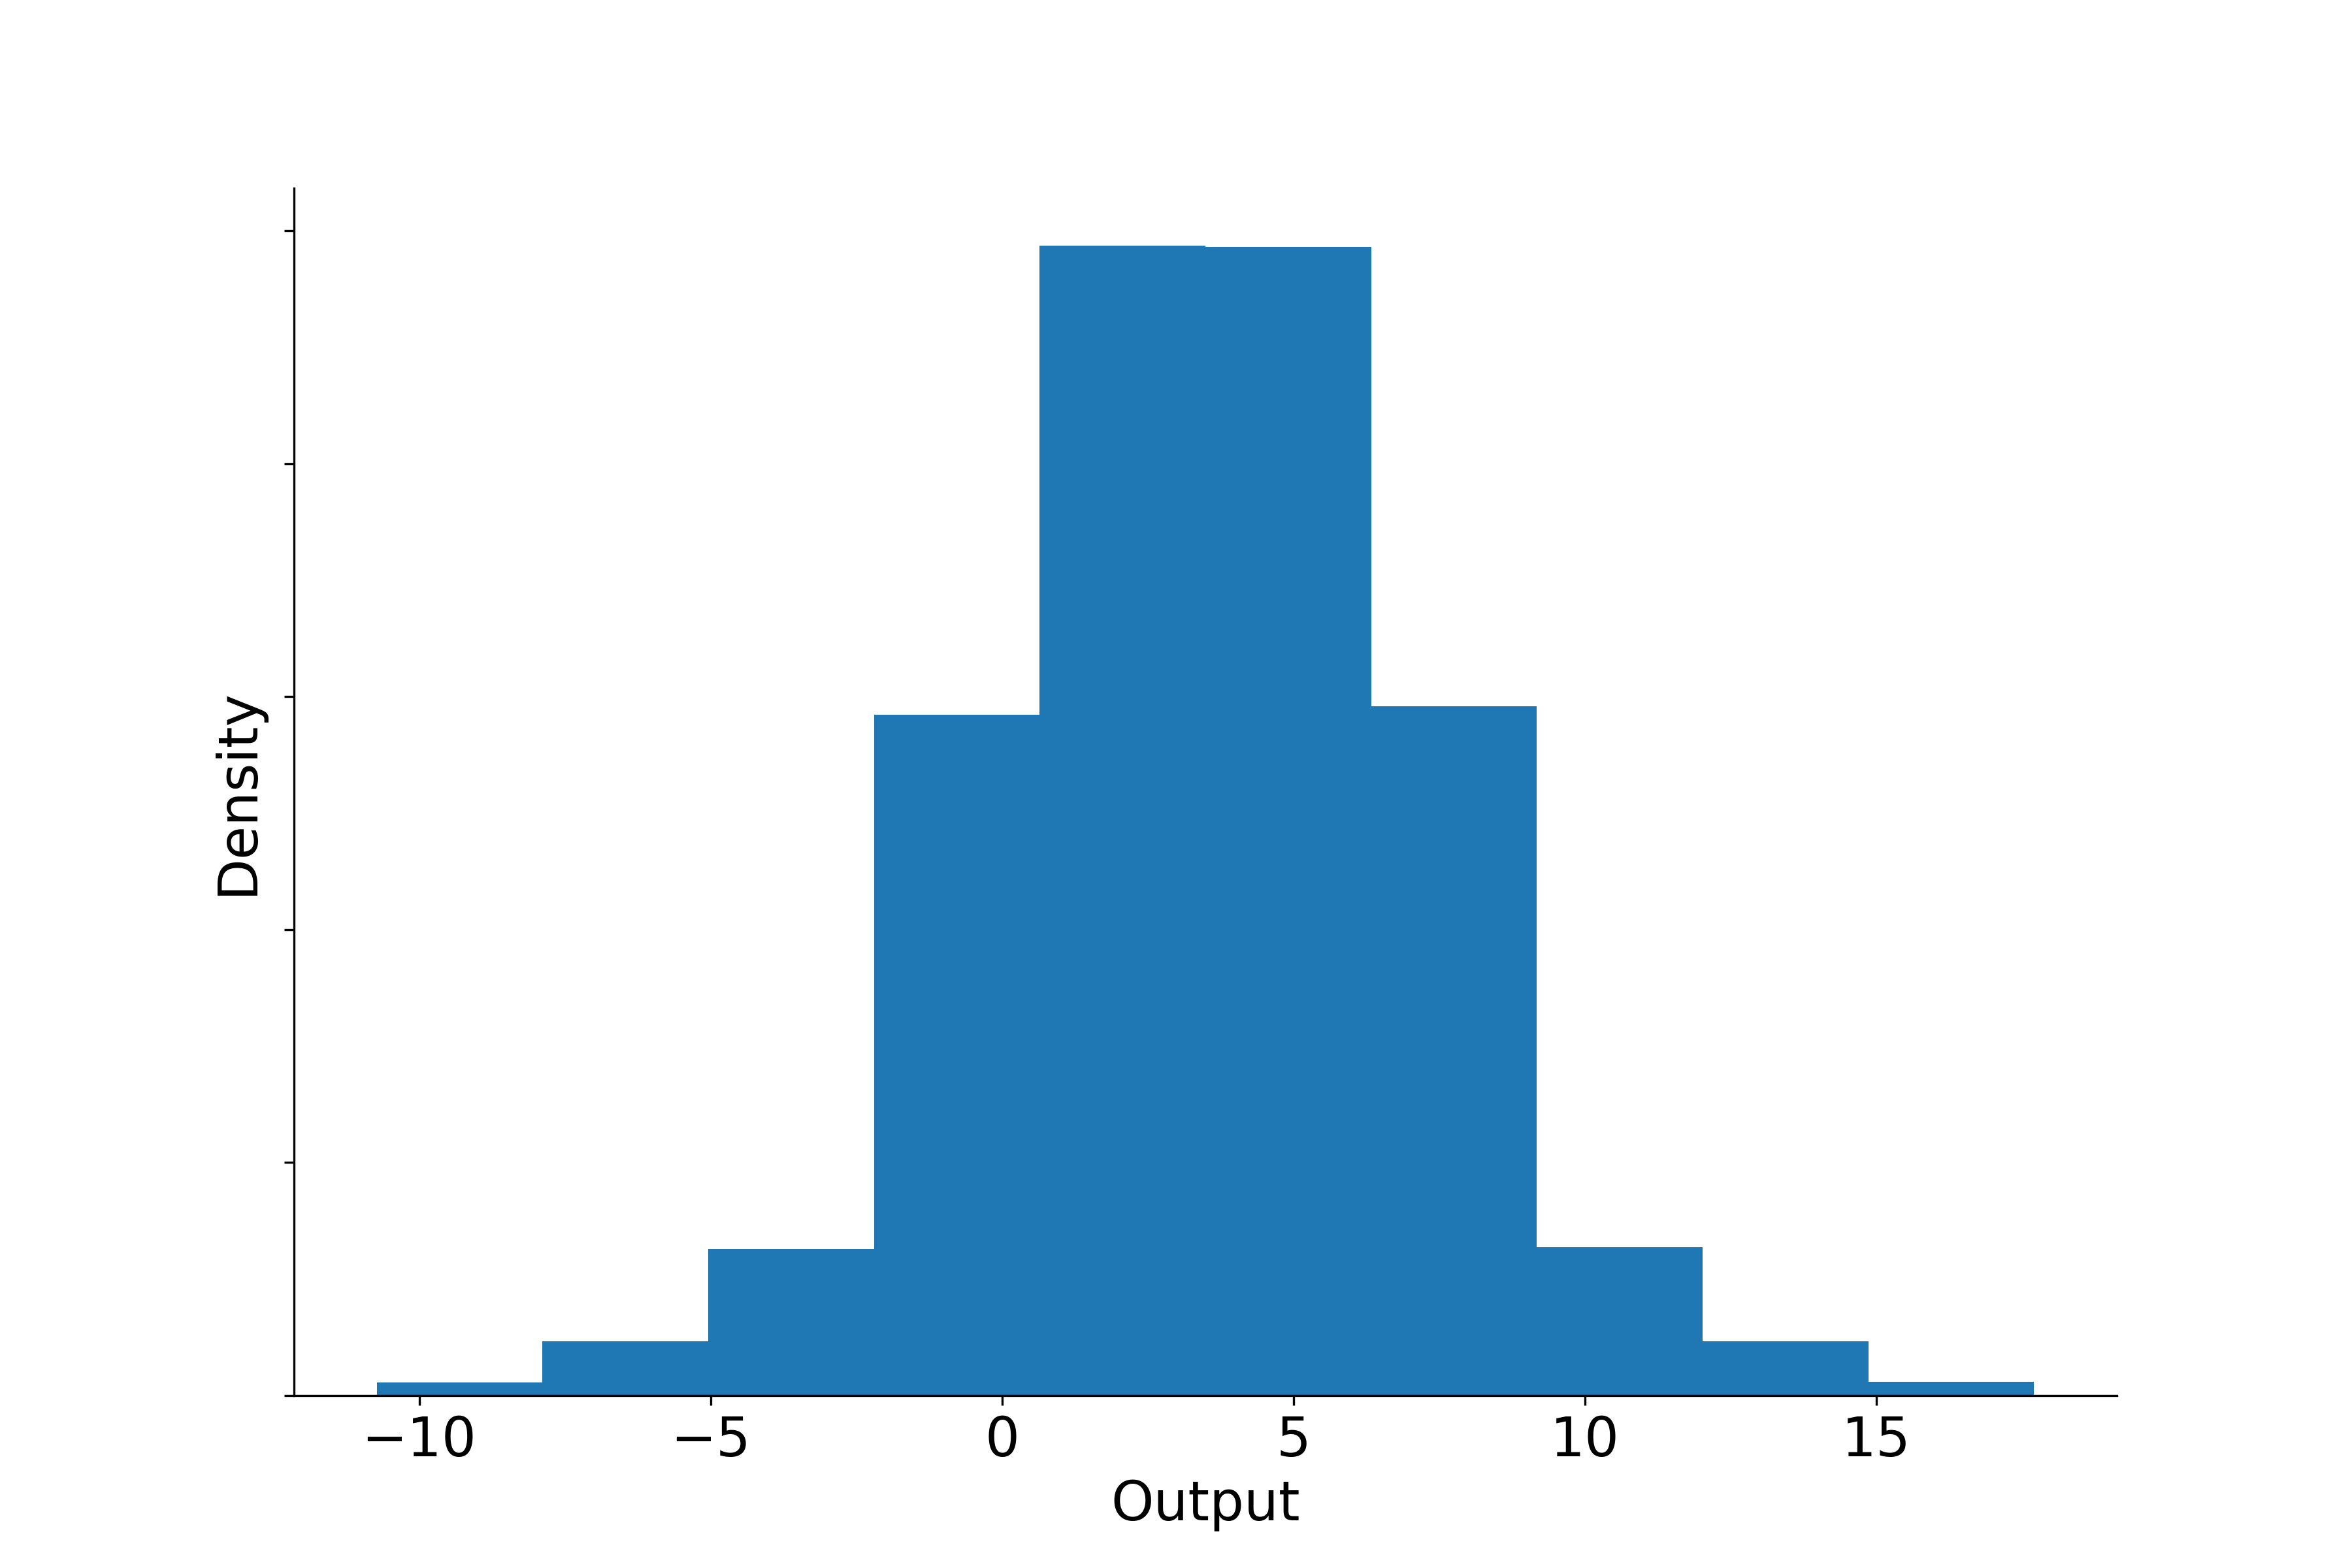
\includegraphics{material/fig-ishigami-uncertainty-propagation}}
\end{figure}
\end{frame}
%-------------------------------------------------------------------------------
%-------------------------------------------------------------------------------
\begin{frame}\textbf{Reference values}\vspace{0.3cm}

\begin{align*}
	\var(Y) = \frac{a^2}{8} + \frac{b \pi^4}{5} + \frac{b^2\pi^8}{18} + \frac{1}{2}
\end{align*}

\begin{align*}
S_1 & = \frac{1}{2} *  \left(1 + \frac{b\pi^4}{5}\right)^2 \; \var(Y)^{-1} \\
S_2 & = \frac{a^2}{8} \; \var(Y)^{-1} \\
S_3 & = 0
\end{align*}


\end{frame}
%-------------------------------------------------------------------------------
%-------------------------------------------------------------------------------
\begin{frame}

\begin{figure}[h!]\centering
\caption{Main effect of input 1}

\scalebox{0.30}{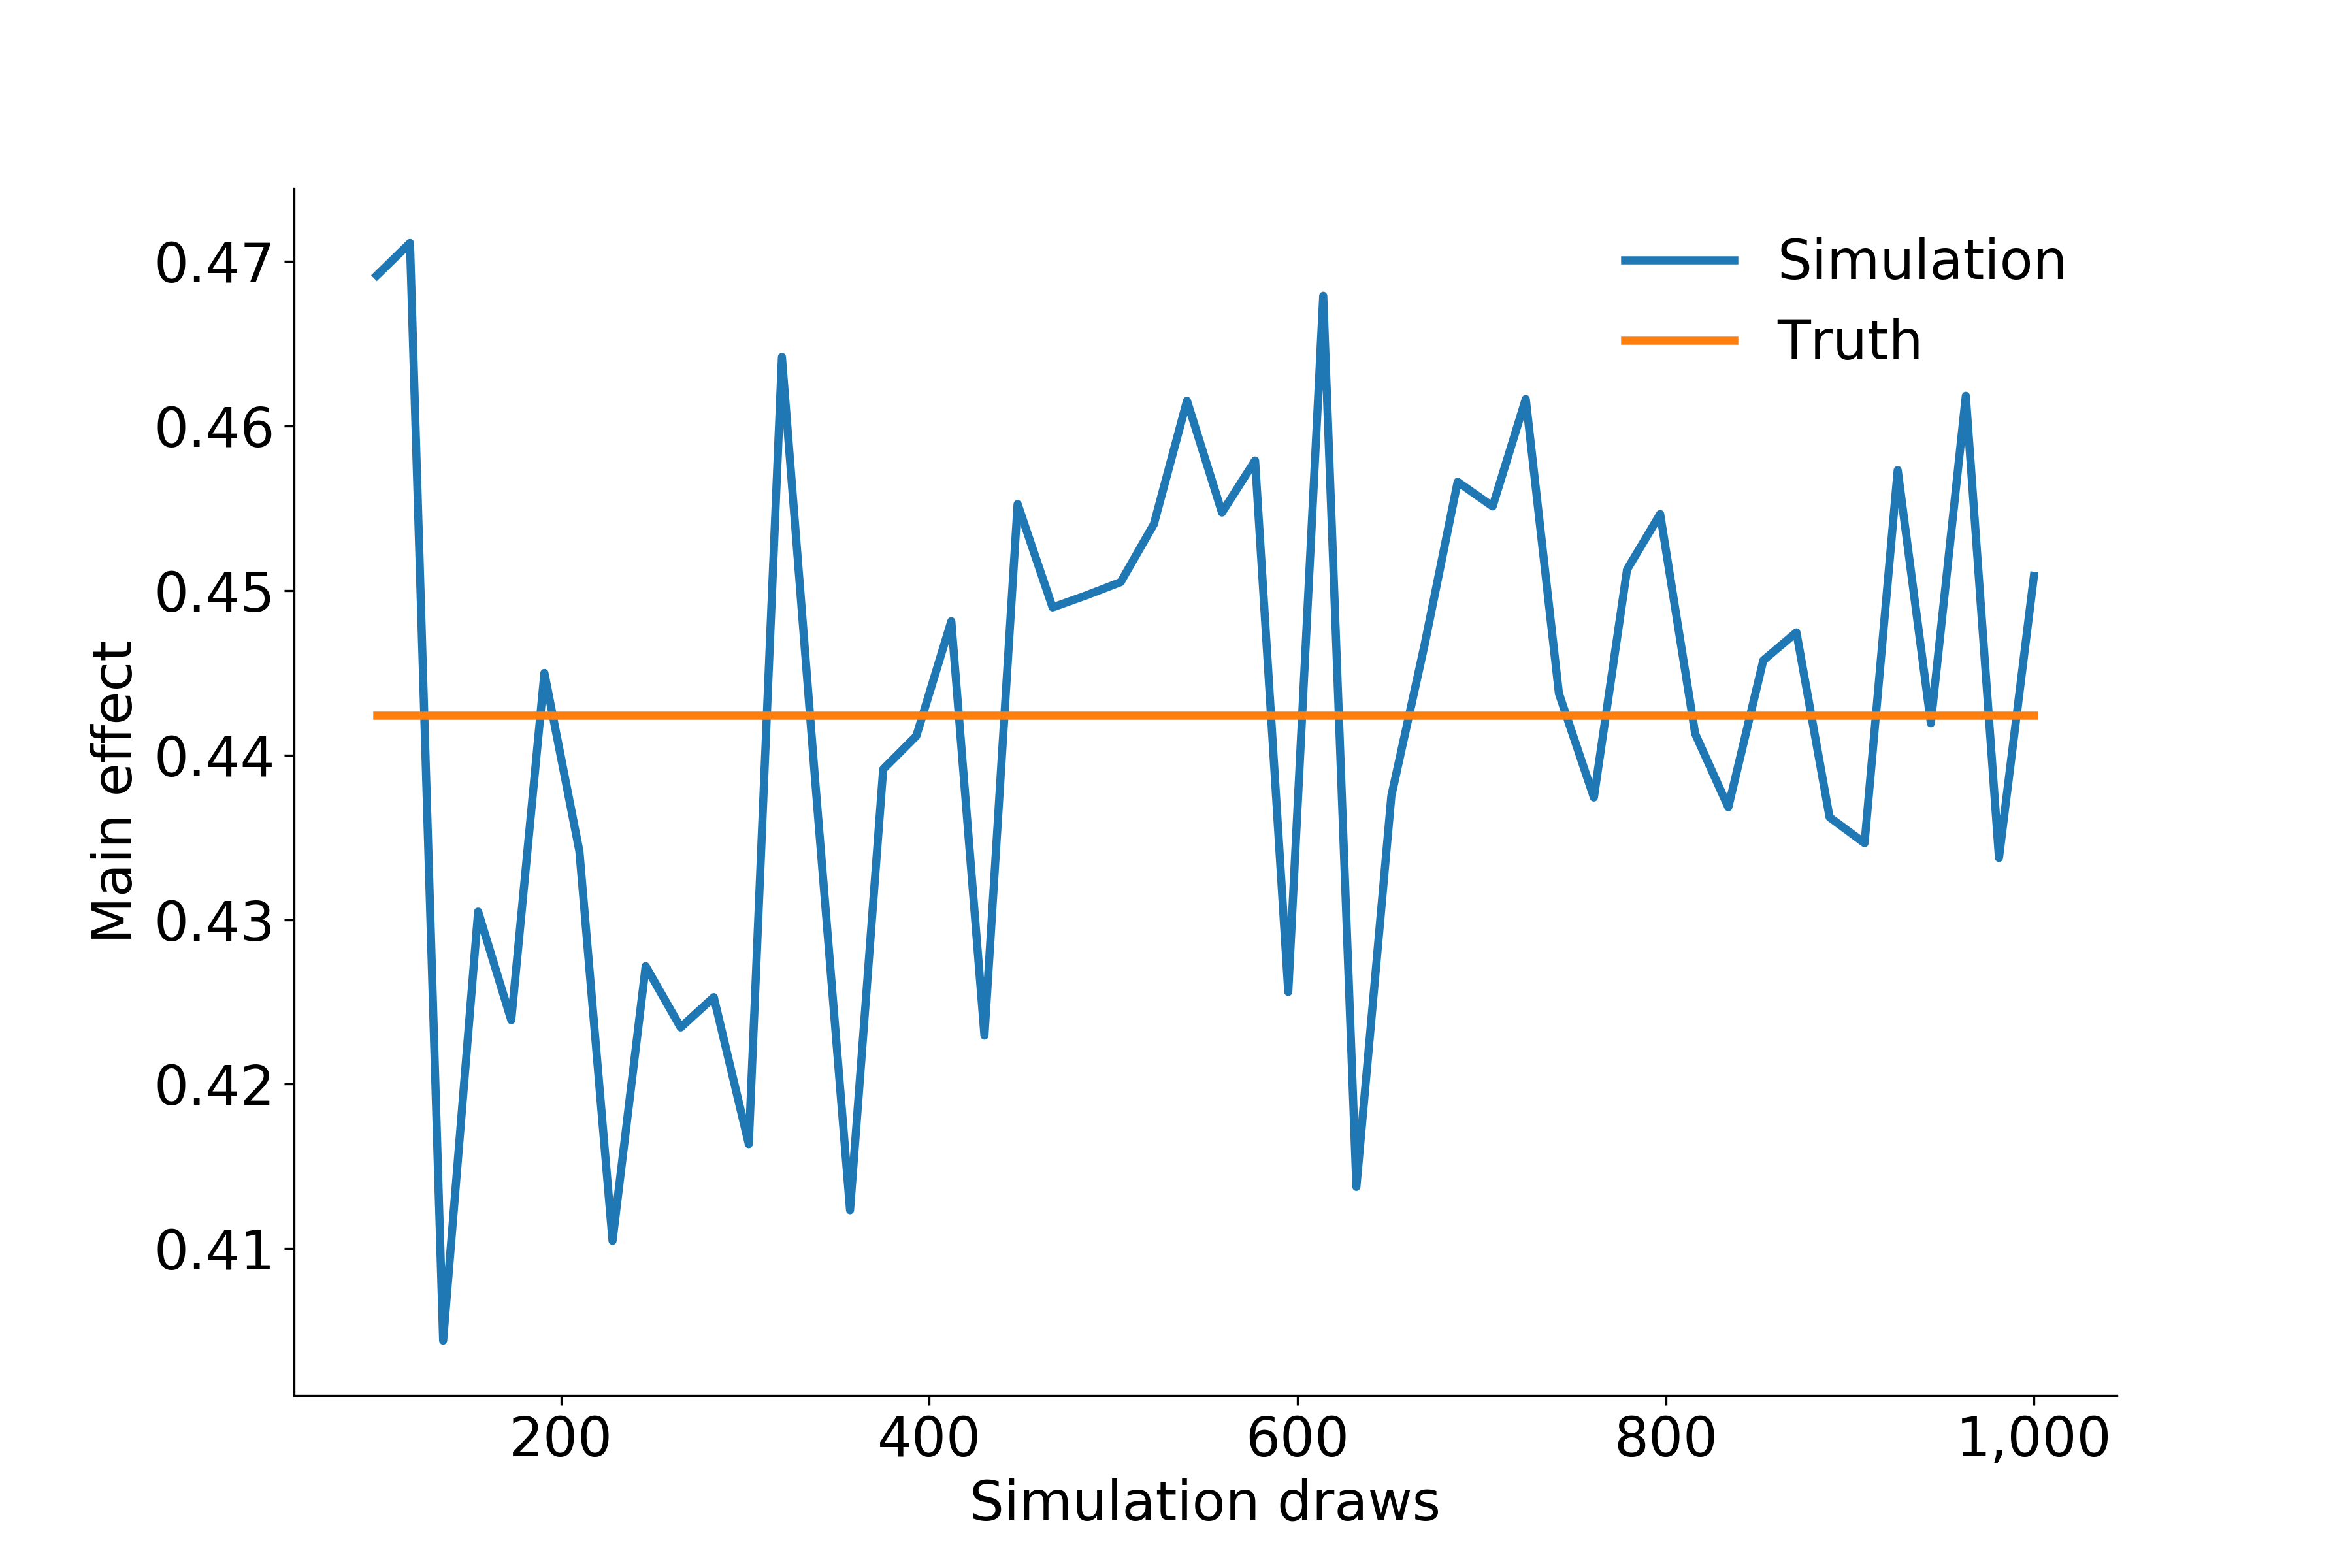
\includegraphics{material/fig-ishigami-main-effect-1}}

\end{figure}

\end{frame}
%-------------------------------------------------------------------------------
%-------------------------------------------------------------------------------
\begin{frame}

\begin{figure}[h!]\centering
\caption{Main effect of input 3}
\scalebox{0.30}{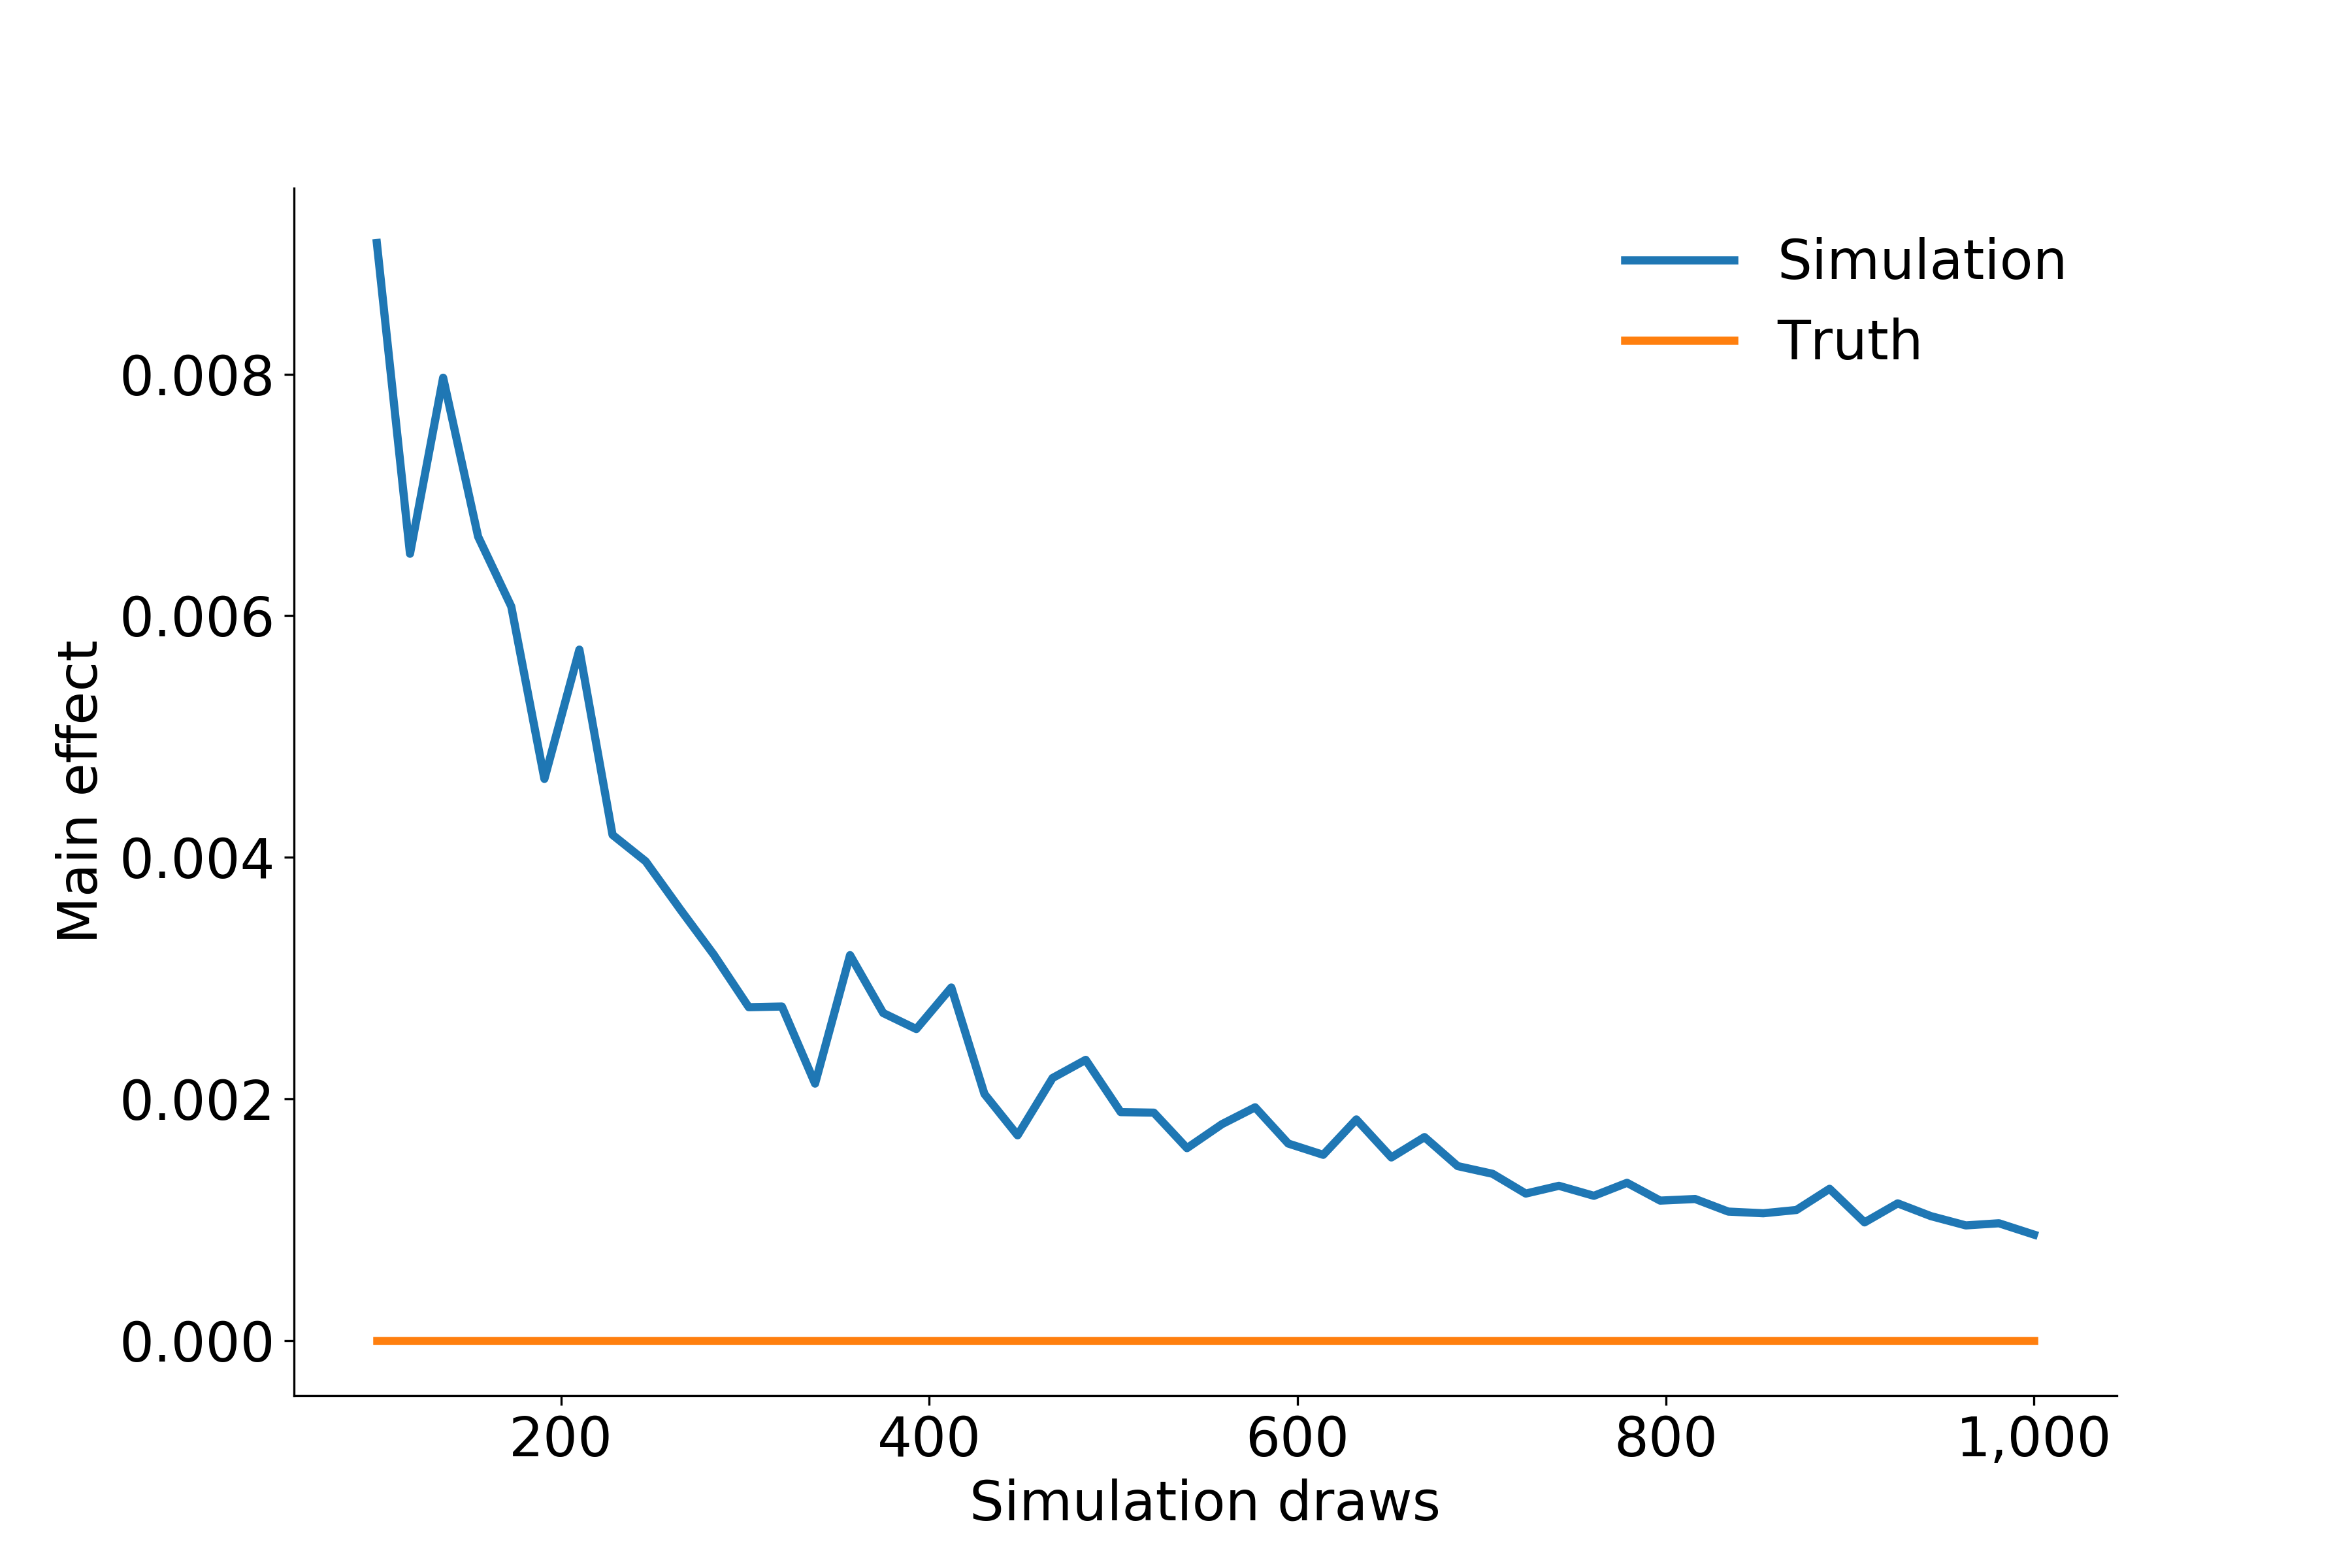
\includegraphics{material/fig-ishigami-main-effect-2}}
\end{figure}

\end{frame}
%-------------------------------------------------------------------------------
%-------------------------------------------------------------------------------
\begin{frame}\textbf{Total effect}\vspace{0.3cm}

\begin{align*}
S^T_1 & = \left(\frac{1}{2} *  \left(1 +  \frac{b\pi^4}{5}\right)^2  +  \frac{8 b^2 \pi^8}{225}\right) \; \var(Y)^{-1}\\
S^T_2 & = \frac{a^2}{8} \; \var(Y)^{-1} \\
S^T_3 & =  \frac{8 b^2 \pi^8}{225} \; \var(Y)^{-1}
\end{align*}


\end{frame}
%-------------------------------------------------------------------------------
%-------------------------------------------------------------------------------
\begin{frame}

\begin{figure}[h!]\centering
\caption{Total effect of input 1}

\scalebox{0.30}{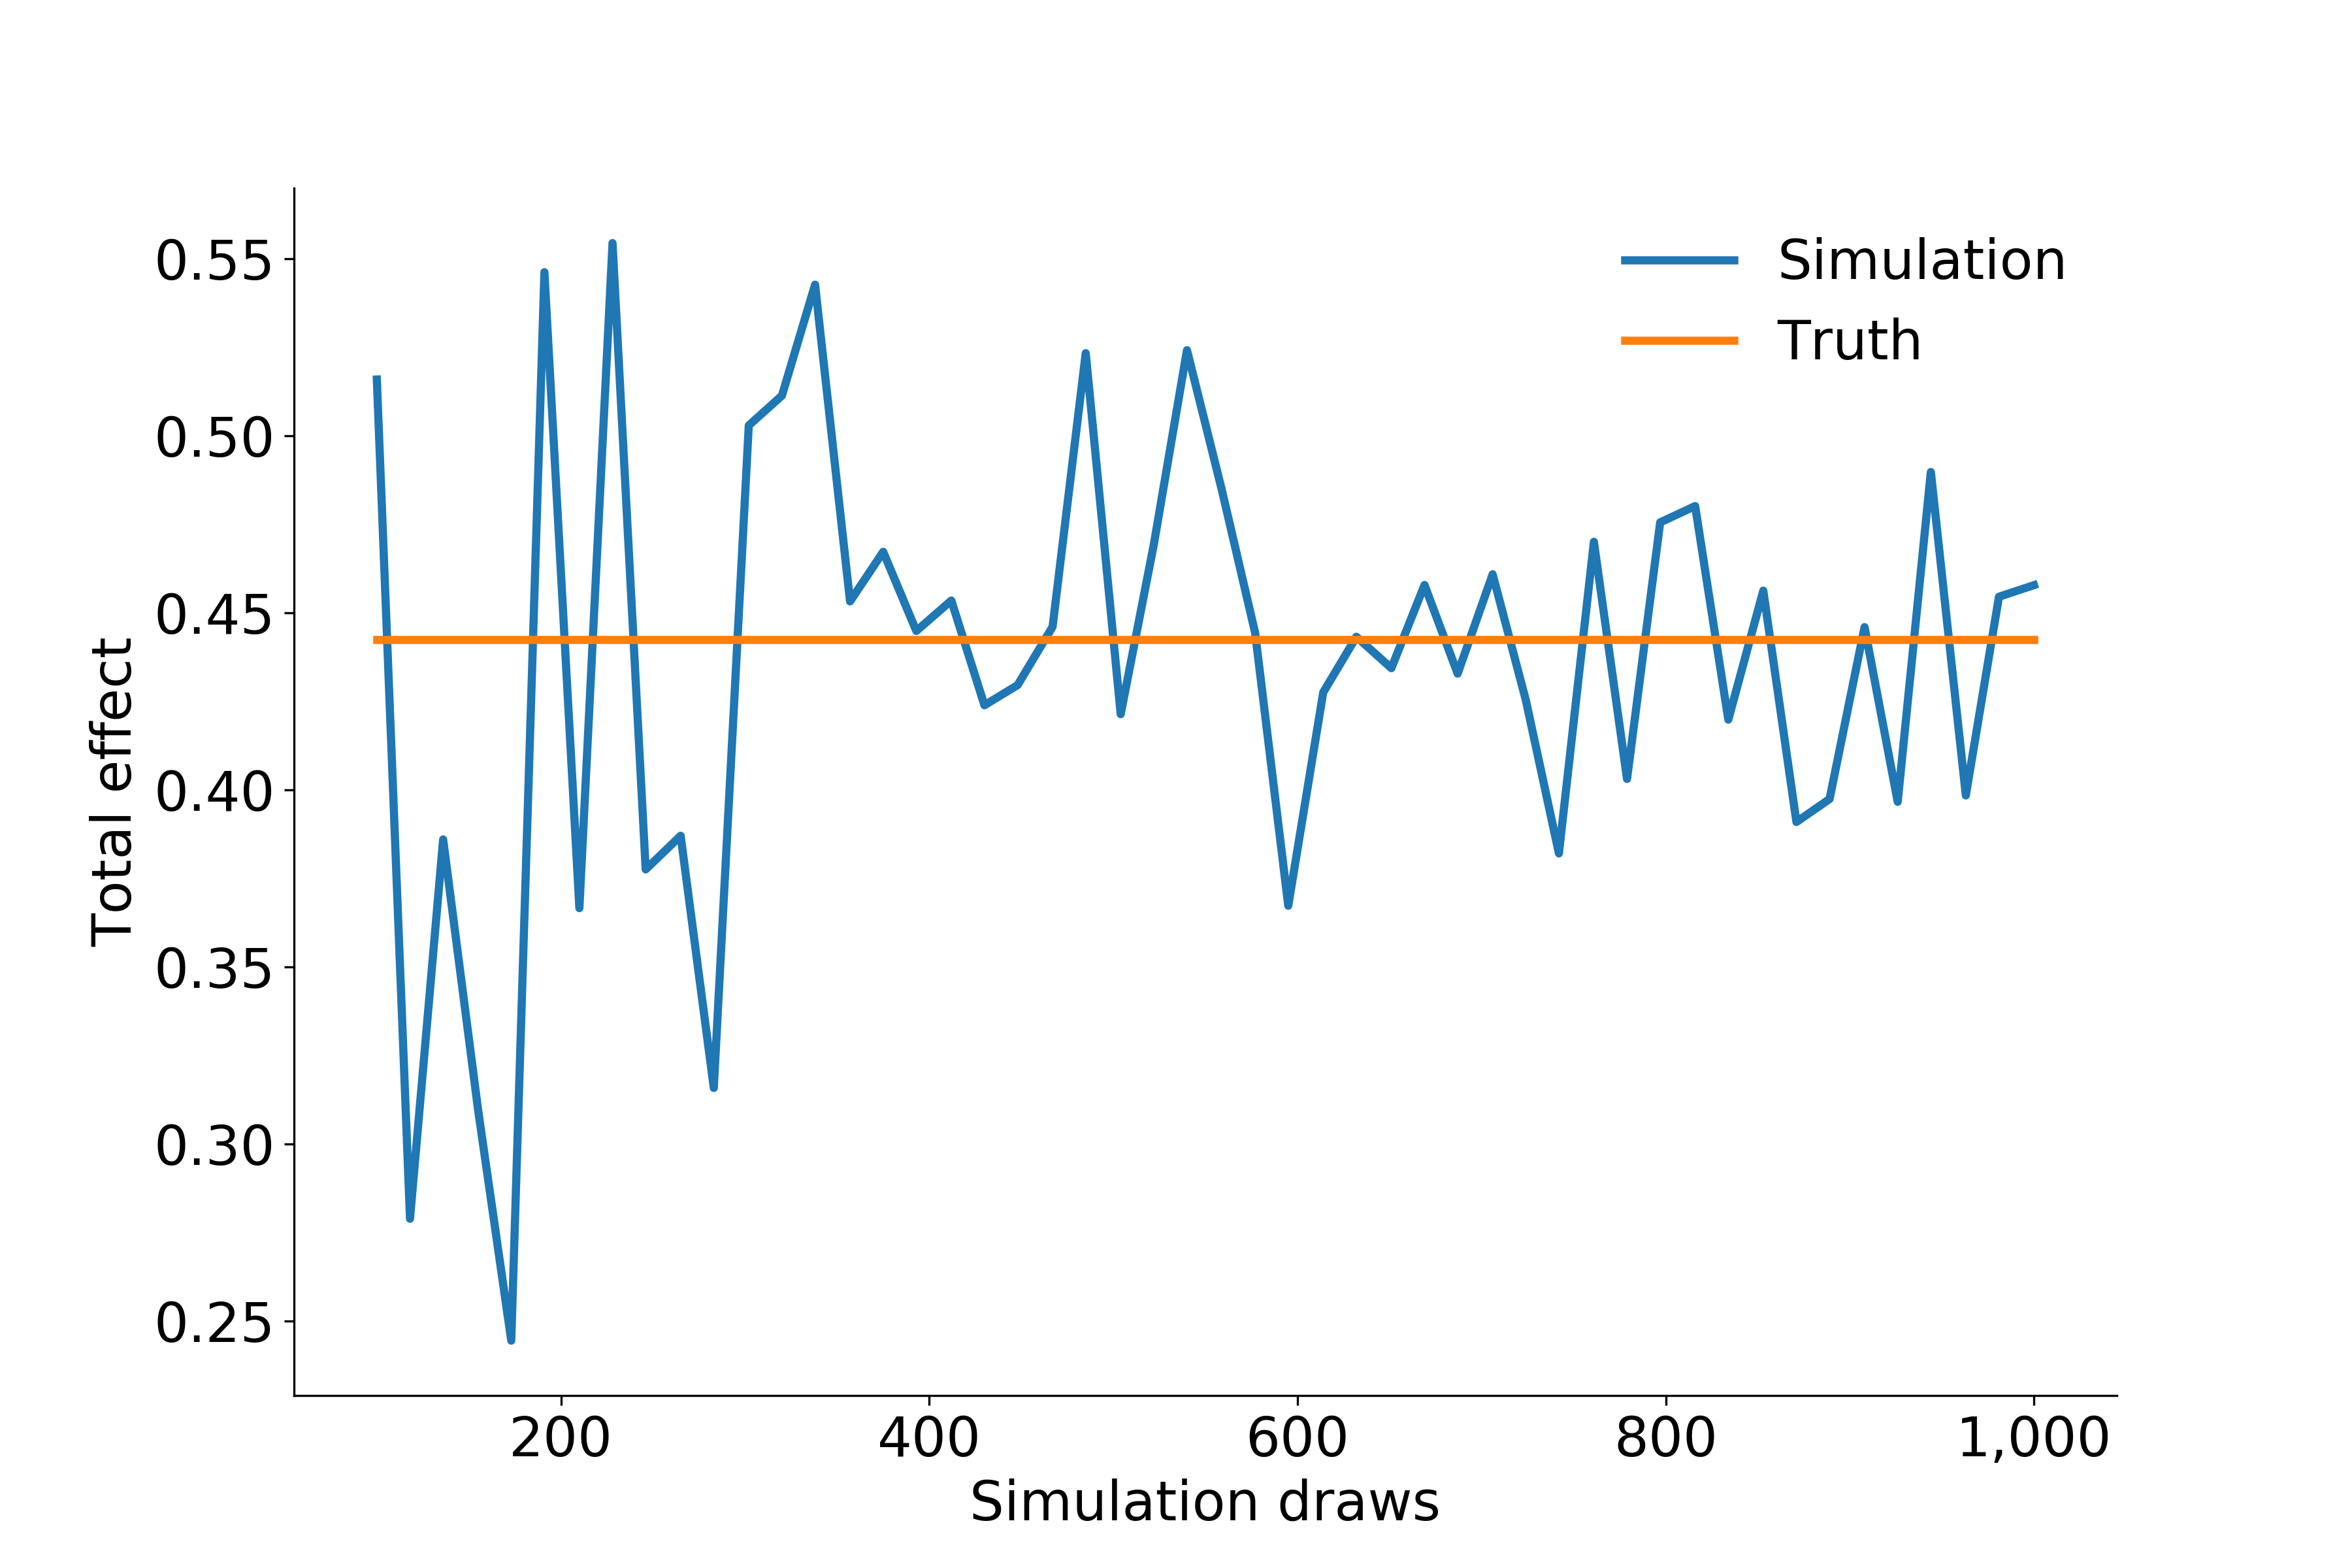
\includegraphics{material/fig-ishigami-total-effect-1}}

\end{figure}

\end{frame}
%-------------------------------------------------------------------------------
%-------------------------------------------------------------------------------
\begin{frame}

\begin{figure}[h!]\centering
\caption{Total effect of input 3}

\scalebox{0.30}{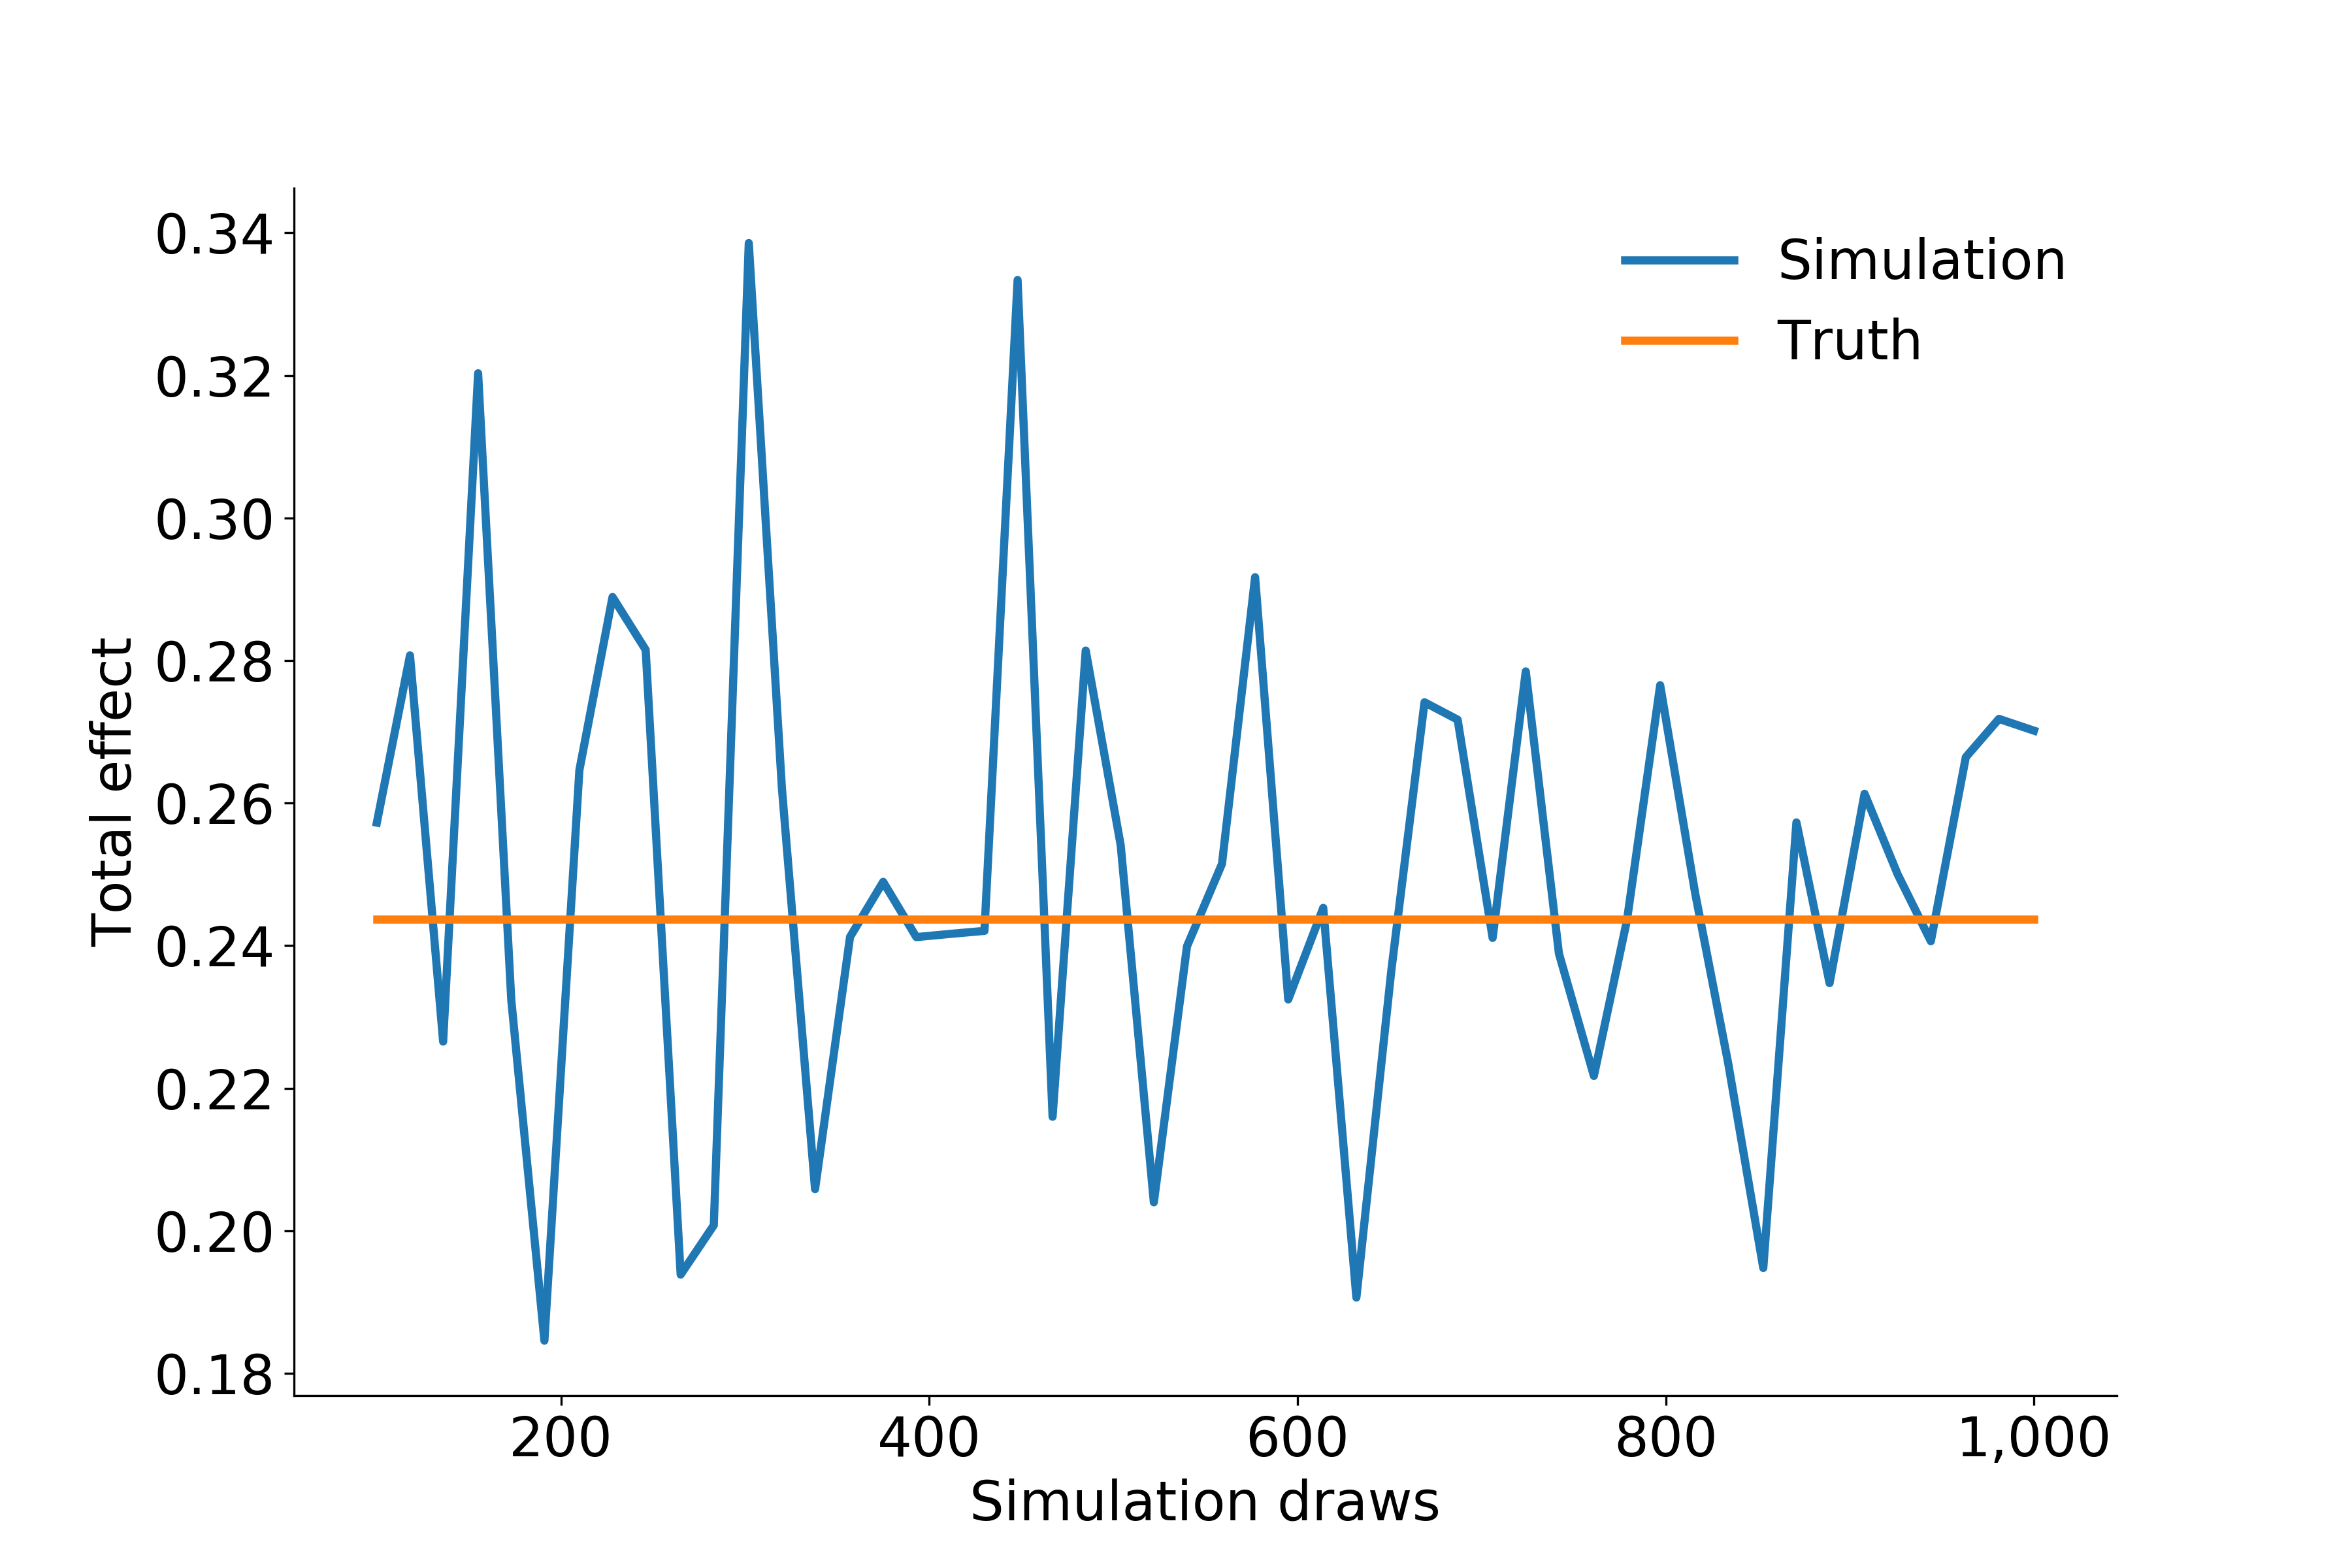
\includegraphics{material/fig-ishigami-total-effect-2}}

\end{figure}

\end{frame}
